\documentclass[a4paper]{article}
\usepackage{pgfplots}
\usepackage[a4paper,top=1cm,bottom=1cm,left=0cm,right=1cm]{geometry}
\usetikzlibrary{pgfplots.groupplots}

\definecolor{BoxCol}{rgb}{0.43,0.62,0.86}
%\definecolor{BoxCol}{rgb}{05686,0.07451,0.07451}
%\definecolor{BoxCol}{RGB}{62,126,148}
\begin{document}
	\thispagestyle{empty}
	
	\begin{figure}[t]
		\centering
		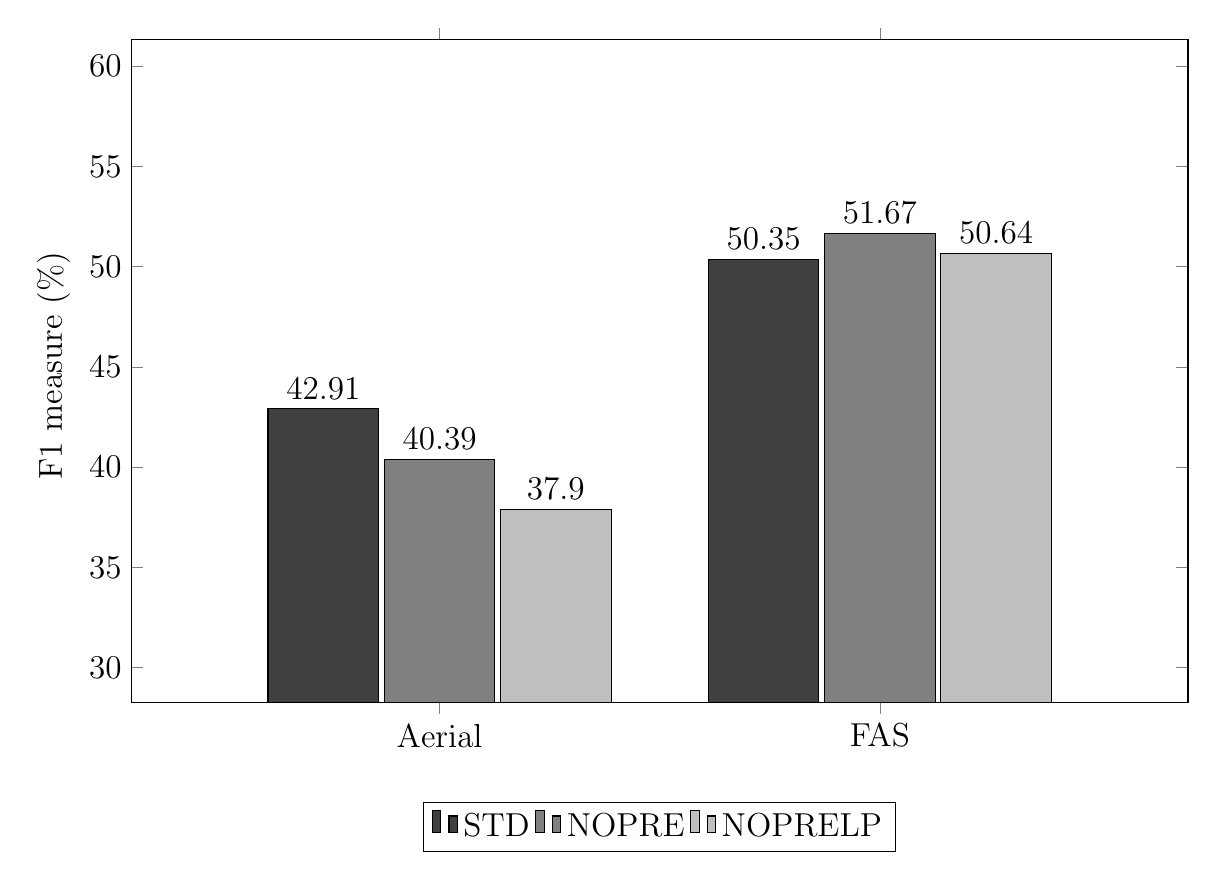
\begin{tikzpicture}
		\begin{axis}[
		width=15cm,
		height=10cm,
		ybar,
		enlargelimits=0.70,
		legend style={at={(0.5,-0.15)},
			anchor=north,legend columns=-1},
		ylabel={\ F1 measure (\%)},
		symbolic x coords={Aerial,FAS,},
		xtick=data,
		nodes near coords,
		nodes near coords align={vertical},
		bar width=40pt,
		style={font=\large}
		]
%					STD		NPRE	NPRE4K
%			Aerial	42.91	40.39	37.90
%			FAS		50.35	51.67	50.64
		
		
		\addplot [color=black,fill=darkgray] coordinates {(Aerial,42.91) (FAS,50.35)  };
		\addplot [color=black,fill=gray] coordinates {(Aerial,40.39) (FAS,51.67) };
		\addplot [color=black,fill=lightgray] coordinates {(Aerial,37.90) (FAS,50.64) };		
		
		\legend{STD,NOPRE,NOPRELP}
		\end{axis}
		\end{tikzpicture}
		
		%\vspace{-0.7cm}
		%\caption{Left: the pitch distribution for the 10 male speakers. Right: the active speech level for the 20 speakers.}\label{fig:pitch}
		%\vspace{-0.5cm}
	\end{figure}
\end{document}